\chapter{Introduction}
\label{chap:introduction}
% \subtitle{Building a distributed reputation system as the basic infrastructure for creating trust 
% between relative strangers for the future digital economy.}

% \paragraph{Abstract.} Trust enables cooperation which in the long-term increases welfare for all 
% parties, but centralization creates an unhealthy information and, thus, power asymmetry. The future 
% digital economy will be driven by global cooperation between relative strangers; that cooperation 
% will be facilitated by distributed reputation systems without central ownership or control. This 
% work extends the scalable TrustChain fabric with an explicit, unambiguous, public representation of 
% the entities' states, thereby making sharing of information incentive-compatbile and putting another
% pillar for the trustful internet in place.

% 1. Since the ground-breaking work of Darwin we know that evolution of species is guided by natural selection, so mutation and inheritance lead to the strongest variation surviving. However, the classic view of the strongest survives does not explain how cooperation can occur, which requires some sort of altruism. Game theory explains …
%  Nowak, Axelrod, 

Trust is the bedrock of society. From the evolution of species, global markets all the way to the 
modern sharing economy, trust has always had an important impact on almost every aspect of our lives.
Trust is built on a good reputation which in turn is created through positive outcomes of past 
interactions. The value of a good reputation also depends on how widely known that reputation is.
In small communities, knowledge about each other is gained through gossiping or personal experience. 
But local communities become less important as global communities and marketplaces become more common
through internet based applications. Still, or even more so, those internet communities depend on 
trust. Protecting and distributing the knowledge about interactions in the digital world is a tough
challenge we are faced with when designing a global trust system.

The current state-of-the-art trust building systems are online platforms for the sharing economy.
The reputation systems of Uber\footnote{https://uber.com} and AirBnB\footnote{https://airbnb.com} are
an essential part of their business. The good reputation allows commuters to trust their driver and
get into the car of a stranger, or allows house owners to rent their home to a couple from the other
side of the world. The reputation of drivers and renters are stored on the platforms, they are both
valuable to the people as well as the company. This leads to problems when renters do not agree with
updates to the platform: they cannot take their reputation and move to a competitor. Users are locked
into those platform, giving platforms great power and influence. 

A similar situation exists in the banking world. Banks are entrusted with their clients money, but 
their power led to corruption and the trust was abused. The situation escalated in the 2007-08 
financial crisis which led to a global recession. The crisis inspired a new solution: Bitcoin. Bitcoin
is supposed to enable secure payments without banks. As such it removes power from financial 
institutions and puts it back into the hands of the actual owners of the money. 

Not every digital money transaction should require a bank, and similarly not every trustful
interaction on the internet should require a third-party. Instead, the ability to prove one's trustworthiness
on the internet should be open and free for anyone. Our vision is therefore to create a universal
mechanism to create trust. This work sets an important 
step towards creating such a system. Specifically we propose a mechanism that protects and 
distributes the records of transaction which are essential for creating trust. 

This first chapter introduces some key concepts around trust and explains the context of this work.
It should shed light on the origin of trust research and its significance for the future of the 
internet. A thorough contextual basis is created for the reader to fathom the problem description
and proposed solution in the following chapters.

\section{Relevant Trust research}
Virtually everyone that is part of a social community understands the concept of trust, yet defining
trust scientifically is hard. This is also due to the fact that trust is studied in a diverse set 
of sciences: evolutionary biology, sociology, economics and lately computer science. In the simplified
form of a model trust can well be described and studied. The prisoner's 
dilemma\cite{chammah1965prisoner} is one such model from game theory that creates a framework for 
understanding trust. It is widely used in research and is the basis for many experimental studies.
We describe in the following the game, it's relation with cooperation and the impact on evolutionary
theory, economics and computer networks.

\subsection{Prisoner's dilemma}
\label{sec:prisoner}
The game Prisoner's dilemma describes a dilemma common in many real-world situations, for
example the problem of two partners caught for a crime that are questioned in two separate rooms. 
Each prisoner has two options, either deny all allegations, which is more generally called cooperating
 or betray the partner, which is called defecting in general game theory. If both stay 
silent, both will get a sentence of one year. If one betrays the other, the snitch is set free while the 
betrayed gets three years in prison. If both betray each other, they both have to serve two years.
When analyzing the game without any additional knowledge and considering the payoffs for one of the
prisoner's it is always advantageous to betray the other. Either the other also betrays, in which case
two years is better than three, or the other stays silent in which case betraying sets us free. 
However, when considering both prisoners' outcomes together it would be best for both to stay silent.


While the game is quite simple the implications are far reaching. The game is able to show the 
connection between trust and cooperation. If both prisoners trust each other to never betray a 
partner, both will cooperate and get a small sentence, the best combined outcome. Yet any mistrust
makes both fail at beating the system. The problem also describes many real world problems, called 
the tragedy of the commons. For example, the global warming is a problem that can only be solved if
all peoples and all nations cooperate. Yet, the low cost and convenient usability of fossil fuels 
make it advantageous to defect and damage the environment. Either the others try to save the environment
in which case a single defection will have a small impact, or the other will also damage the environment
in which case a single cooperator will fail anyways. Only, if everyone trusts each other that
everyone does the best they can to save the environment, then it is possible to beat the tragedy 
of the commons.

\subsection{Evolution and cooperation}
\label{sec:evolution}
While cooperating, according to theory, is not necessarily a winning strategy, it is in our nature 
to do so, as has been shown by evolution theorists. The theory about competitive natural selection 
between individuals and mutation and inheritance of genes was the accepted truth about evolution 
since Darwin until in the late 1960s doubts arose about the completeness of this 
theory. When looking at group behavior in species one will find that cooperation is a common theme
among related individuals, yet there is no place for cooperation in the classic Darwin 
theory~\cite{Axelrod1390}. In their work Axelrod and Hamilton \cite{Axelrod1390} 
analyze how to combine the seemingly inferior individual's strategy of cooperating with the goal to 
maximize fitness. At the basis of their experiments is a again the Prisoner's 
Dilemma. Axelrod and Hamilton ran experiments on this game with multiple rounds instead of only one with
different strategies. They found that if the game is played repeatedly with the possibility of 
meeting the same partner again in the future, cooperation between players can be established and be
superior. Later research showed that this direct form of reciprocity, the act of returning a deed,
is only one form of cooperation found in human behavior. Nowak and 
Martin~\cite{nowak2006five} defined in total five forms in which cooperation can occur: kin selection, direct
reciprocity, indirect reciprocity, network reciprocity and group reciprocity. Conceptually these 
forms can be described like this:

\begin{itemize}
    \item kin selection: we help those that share our genes
    \item direct reciprocity: I help you, you help me
    \item indirect reciprocity: I help you, somebody helps me
    \item network reciprocity: neighbors help each other
    \item group selection: A group, in which members help each other, survives
\end{itemize}

Each concept entails at its basis trust. We trust our family, our group, our countrymen, those with whom we had a lot
of shared experiences and those we heard good things about. 
% 2. Trust in economy and digital markets …. Advance of sharing economy, ….. When talking about trust, indirect reciprocity is the method of creating cooperation. Mui created a first mathematical model which relates reputation, trust and reciprocity. According to that model reputation stems from the history of encounters 
% Mui, Martin

\subsection{Economics}
{\color{red} Old: needs to be improved}
Trust also plays a major role in our economic system and has been for the the evolution of economy 
as shown in Figure \ref{fig:economy}. In the pre-industrial age, most economy and trade was done in local
communities with families that trusted each other over generations and traders that returned year
after year. During industrial and post-industrial age companies have largely replaced local 
producers and are trusted by millions of customers based on their brand name. Nowadays, in the 
information age, internet companies allow people to connect, trade and cooperate directly, examples
being eBay for trading physical goods, AirBnb for sharing houses and Uber for ride-hailing. How trust
and the lack of it influence trade and markets has been studied in the well-known paper by 
Akerlof~\cite{akerlof1970lemons}. He describes the information asymmetry between seller, who knows
the quality of the goods which will be sold, and the buyer, who can only estimate that quality by 
some market statistic. The seller's incentive to sell goods of lesser quality than the average 
statistic leads to a decreasing statistic and thus price which in turn decreases the quality of the 
goods sellers are willing to offer for that lower price. Hence the market breaks down. Akerlof
describes institutions to solve this problem namely institutions such as guarantees, brand names and
certifications. These are trust inducing institutions and can be generalized as reputation systems.
If the sellers sell goods to many people and those people report or gossip the good quality of what
they have bought, others can trust those sellers and both seller and buyers will thrive. On the 
other hand a bad reputation will lead to a seller getting out of business as buyers will mistrust.
This closes the gap to the work of Nowak as this reputation is what makes indirect reciprocity
possible: the seller is not taking advantage of the buyer's inconvenient situation but the buyer
cannot directly return that favor. Only by gossipping the event to other potential buyers who are 
then more willingly to buy from the seller is the reciprocity circle closed.~\cite{nowak2006five}

\begin{figure}[t]
    \centering
    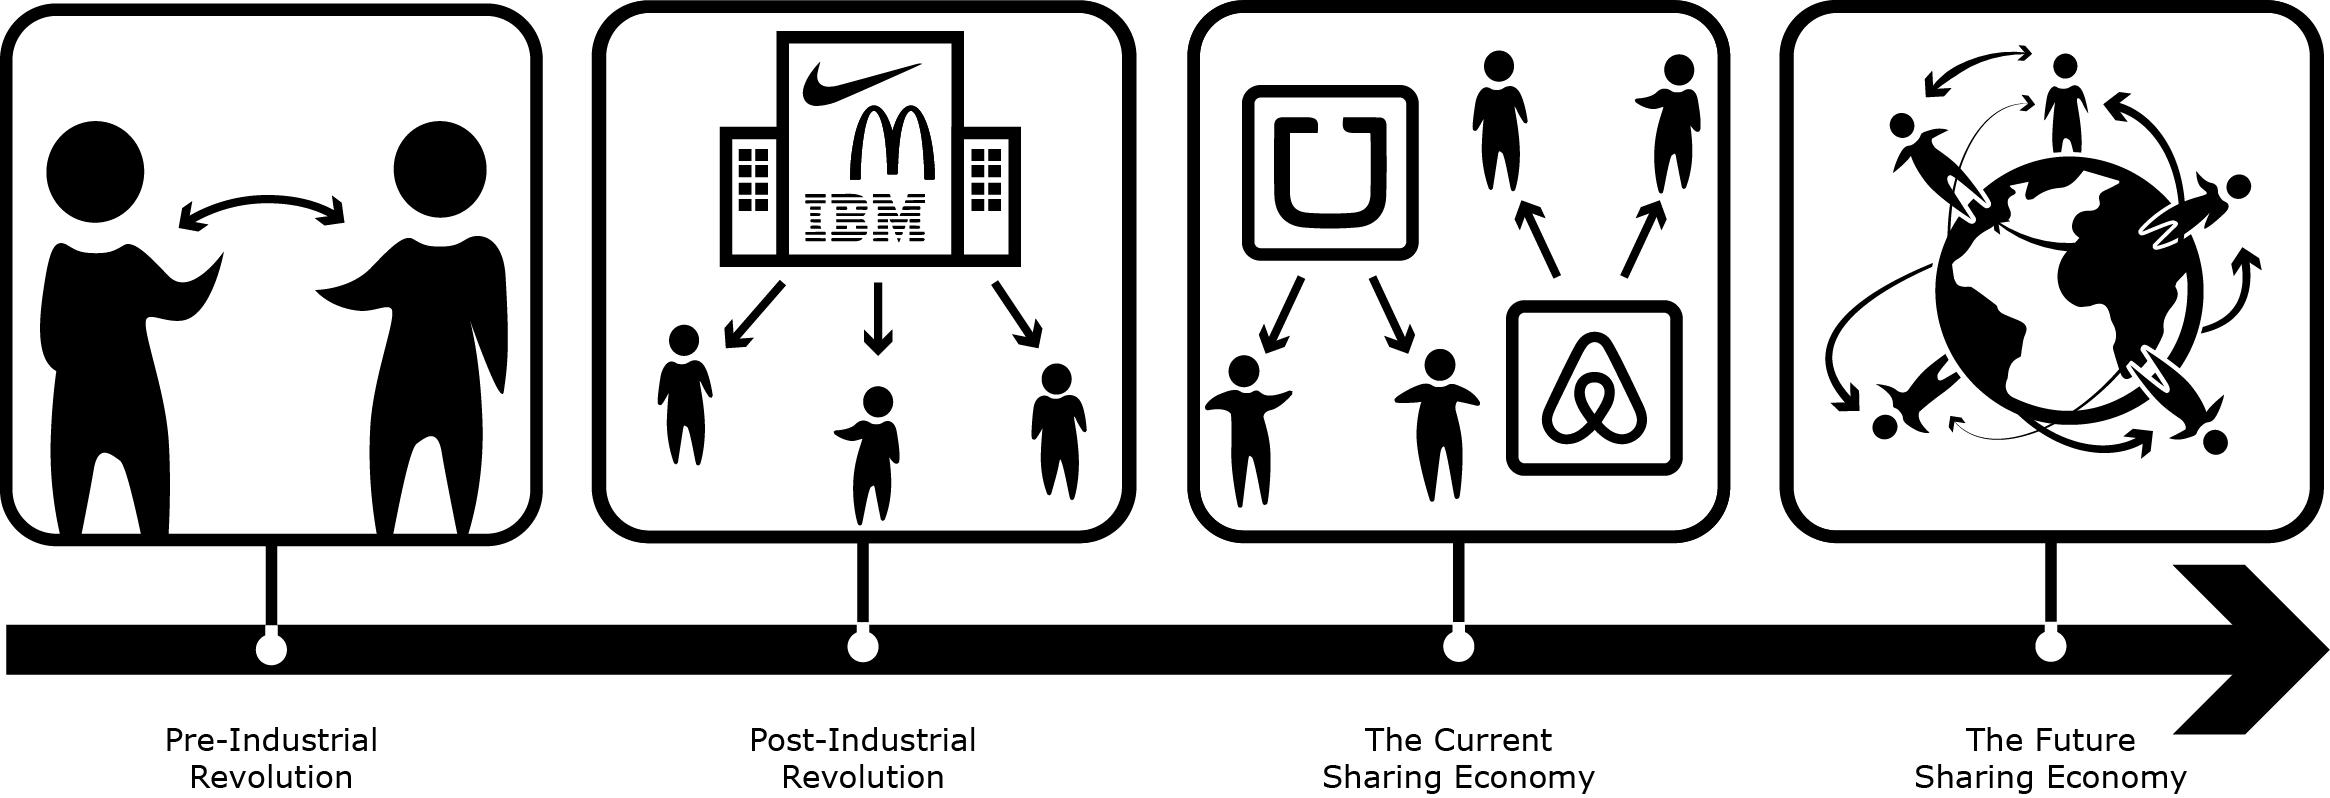
\includegraphics[width=0.8\textwidth]{images/economy.png}
    \caption{Evolution of the economy}
    \label{fig:economy}
\end{figure}

% 3. Reputation systems guide buyers towards to most trustworthy sellers on markets or help guests find houses on Airbnb that actually hold the promises made in the description. Reputation systems require three properties: dissemination, strong identities and  Yet companies take advantage of our trust and misuse our data, influence us and do not take appropriate measures to protect our data from attacks. Centralized systems are broken.
% (eBay) Ba and Pavlou, survey of reputation systems, definition of reputation system, Pouwelse 
\section{Digital trust}
{\color{red} Old: needs to be improved}
These analog, gossip-based reputation systems are what guide our decisions in buying cars, new or 
used, at which bank we store our money and at which restaurant we should have dinner.
But reputation systems are also prevalent in the digital world: we make our decisions in buying used goods 
on eBay, renting a house to a stranger (or from a stranger), getting into a stranger's car 
(what mum told us not to) based on the reputation of the partner. The sharing economy or collaborative consumption is the 
rising star of economic concepts in the information age and it is power by reputation. A company 
offers a platform on which the two sides of a trade or transaction can find each other. With each 
encounter both parties can rate that interaction and it becomes part of their history. With a longer
and more positive history the value of a profile increases as users see the reputation as security
for a good interaction and are willing to pay for it. However, there are reasons for concern. What
if the platform changes their rules in an almost unacceptable way or abuses the personal data their
users have entrusted them with? Users cannot take their reputation and data to another platform
because their reputation is actually owned by the platform facilitating the trades. Such abuses
in which trusted companies act wrongly have been happening in many times in the past, examples being
the dieselgate~\cite{VWDiesel} and the facebook/cambridge analytica scandals.~\cite{facebook} These
scandals show that even though millions of users trust them, central institutions do not necessarily
serve their customers or clients. 

% 4. The above discussion makes clear that the future digital economy requires a distributed reputation system. But making a reputation system distributed brings many additional challenges. A distributed system has no control entity which can enforce strong evidence for identities. Also single entities in a distributed system have most commonly no full view of the network, thus are not aware of all other entities or all encounters. The field is not entriely new but distributed reputation systems have been researched especially in the context of peer-to-peer file-sharing, and mobile ad-hoc system. Donation game is the game-theoretic model for this …. Although a lot of research has been conducted in the field of distributed reputation systems, major problems like the Sybil-attack, double spending, scalability and state consistency remain largely unsolved.
% Game-theoretic modeling of reputation
\section{Universal mechanism to create trust}
{\color{red} Old: needs to be improved}
We envision a future in which collaborative consumption is possible without any intermediator. This
future requires a reputation system which is application agnostic, owned by noone and ruled by 
everyone. A distributed reputation system as a layer directly
on top of the internet. However this poses some challenges from a technical
point of view. Distributed system are intrinsically hard to control and regulate, which is both 
blessing and curse. No party can impose unfair rules on other users but it is also hard to prevent 
malicious users from sending wrong information across the network. \cite{HENDRIKX2015184} reviews
state-of-the-art reputation systems and finds that all commercial reputation systems are centralized.
Some of the scientific reputation systems are decentralized like EigenTrust 
\cite{kamvar2003eigentrust}, P-Grid \cite{aberer2003p} and RateWeb \cite{malik2009rateweb}, yet
they have not been proven to work in settings where high throughput, global scaling are required 
which is the case for a global reputation system. Distributed, secure and globally scalable systems
remain an unsolved problem.

% 5. This master thesis was written in the context of the blockchain lab at TU Delft which has a long history of research on the topic of distributed reputation systems. The research is targeted at Tribler, a secure BitTorrent client which is aimed at protecting against free-riders.
% BarterCast

\section{TU Delft Blockchain Lab research}
The ambition of creating the first global trust system is realized at the Blockchain Lab of TU Delft,
which is the research group in which this thesis was created. The lab has a strong focus on exploring
new concepts, implementing them and testing them in production grade software. 

The research group has great experience and a solid track record in the field of distributed work 
systems. Especially peer-to-peer file sharing system have been studied, first and foremost the 
internally developed Tribler\footnote{https://tribler.org} application. Tribler is a client for the
BitTorrent protocol. It offers many improvements over conventional BitTorrent clients like improved
privacy and security, streaming and reputation management. It has been the testbed for algorithms of
bachelor, master and Phd students for ten years with 1 million downloads in that period. In those 
years of research several milestones have been reached. In \cite{meulpolder2009bartercast} we have 
solved the free-riding problem in the peer-to-peer file-sharing context with a reputation system 
that tracks uploads and downloads. With TrustChain \cite{OTTE2017} we have created our own 
blockchain fabric for bandwidth as a currency which builds on the previous work and adds 
tamper-proof recording and immutable history to the reputation system.

The problem of peer-to-peer file sharing systems maps well onto the trust domain. Users of BitTorrent
clients download from other users who upload data. Downloading data has benefit to users because 
they are interested in the content, however uploading has no obvious advantage. It is only necessary
to keep the content available for others. There is an obvious incentive problem, a tragedy of the 
commons. A free-rider can download without uploading, thereby consume resources without contributing.
The problem can be solved through a trust system. By recording the behavior of each user and making
it public a reputation can be assigned to each user which represents their resource usage. Users 
that contribute a lot increase their reputation while downloading decreases that reputation. Other 
users are able to inspect that past behavior of any potential partner and use it for their decision 
whether the partner deserves a contribution. 

The recording of file transactions and security of those records is facilitated by our blockchain
fabric TrustChain~\cite{OTTE2017}. TrustChain is a multi-chain fabric which lets each user create
an own chain. It is therefore built for horizontal scalability and unbounded throughput. By design,
TrustChain enables the creation of trust in any application context. The solution is implemented
in Tribler and has been used in production for more than a year as of 2018. The implementation 
details of TrustChain will be discussed more in Chapter~\ref{chap:model}. 

The great scalability of TrustChain comes at the cost of security. The architecture allows for 
attacks to be detected but the system can only be secured if honest users engage in that defensive 
behavior. This can only be ensured through incentives: agents should never be able to gain an 
advantage by circumventing the rules. 

\section{Contribution}
In this work we study a mechanism to ensure the proper dissemination and verification of transaction
records. In any trust system, the transaction records are the basis for the reputation of users and 
thus the trust users have in each other. With the records, also the reputations itself are spread, 
leading to more agreement of reputation and thus higher value. Also defending the reputation records
against attacks makes records more credible and dependable, opening applications for TrustChain with
higher requirements for security.

We will enlarge on the problem description in the next chapter. Afterwards the problem will be defined
formally and analyzed in the bounds of the definition. Before proposing a solution, some existing
approaches for recording and dissemination of data will be discussed in chapter. Next, we define a
solution based on the TU Delft blockchain fabric TrustChain and propose a specific mechanism of 
using such a fabric. Finally, we prove the correctness and scalability properties of the fabric in
experimental analysis, before concluding and making suggestions for further research.